\documentclass[10pt]{article}
\usepackage[utf8]{inputenc}
\usepackage[T1]{fontenc}
%\usepackage[danish]{babel}
\usepackage{amsfonts}
\usepackage{amsmath}
\usepackage[pdftex]{color,graphicx}
\usepackage{fancyhdr}
\usepackage{textcomp}
\usepackage{lmodern}
\usepackage[table]{xcolor}
\usepackage{multicol}
\usepackage{multirow}
\usepackage{soul}
\usepackage{algorithmic}
\usepackage{graphicx}
\usepackage{wrapfig}
\usepackage{float}
\usepackage{lastpage}
\usepackage[a4paper]{geometry}
%\usepackage{hyperref}
\pagestyle{fancy}
\newcommand{\HRule}{\rule{\linewidth}{0.5mm}}

%If in need of a header for the document, uncomment this and add desired text!
\fancyhead[L]{Exam Notes Datanet}
\fancyfoot[L]{}
\fancyfoot[C]{}
\fancyfoot[R]{\thepage \ of \pageref{LastPage}}
%%%%%%%%%%%% END OF PREAMBLE %%%%%%%%%%%%%%%%%%%%%%%%%%%%%%%%%%%%
\begin{document}
\begin{titlepage}

\begin{center}
\textsc{\LARGE Exam Notes Datanet}\\[1.5cm]
\HRule \\ [7.5cm]
% Author and supervisor
\begin{minipage}{0.5\textwidth}
\begin{flushleft} \large
Martin Grünbaum \\
\textit{martin@itsolveonline.net}\\
\end{flushleft}
\end{minipage}
\begin{minipage}{0.4\textwidth}
\begin{flushright} \large
\textbf{\today} \\
\end{flushright}
\end{minipage}
\vfill
% Bottom of the page front page

\end{center}

\end{titlepage}
\newpage
\thispagestyle{empty}
\tableofcontents
\newpage
\setcounter{page}{1}
\section{Packet-switched networks}
Packet switched networks differ from circuit-switched
networks in that they do not guarantee bandwidth by dedicating
a connection to the purpose. 

Packets are data that you want to send through the system, possibly
split up into many smaller packets, to fit within the size constraints
of routers and switches.

\subsection{ISPs}
There are usually 3 tiers of ISPs:
\begin{enumerate}
    \item Tier 1 ISPs, directly connectd to other tier-1 ISPs. International.
        \subitem Known as the Internet backbone. Sprint, Verizon, etc.
    \item Tier 2 ISPs, which are connected to a/a few tier 1 ISPs
        \subitem Typically provides regional coverage.
        \subitem 'Customer' of a tier-1 ISP
        \subitem Has end-point customers ('real' customers)
    \item Tier 3 and below
        \subitem Even more regional usually, and will connect to the tier
        above.
\end{enumerate}

Tier 1 forms the backbone of everything, and tier-2 connect directly to those
and will have customers. Its like leasing out a cable, and a sub-section of it
is then leased on to someone else, who then leases on a subsection of that seciton.

\subsection{Delay / Loss / Throughput}
\subsubsection{Processing delay}
Time required to examine a packet's header, and determine where to direct the
packet. Microseconds or less.

\subsubsection{Queueing delay}
The delay before a packet is transferred into the limited-space queue of the
link. 

\textbf{Traffic intensity} = La/R where: \\
L = packet size\\
a = average arrival rate of packets\\
R = transmission rate\\

If La/R is over 1, then the queue will increase without bound, because you're
getting more incoming traffic than you're pushing out.

\textbf{Packet loss} occurs when the queue is 100\% full, at that point the
packet is dropped.

\subsubsection{Transmission delay}
The delay to push all of the bits of a packet onto the link, measured as L/R
where L is the size in bits and R is the transmission rate in bits/second.

\subsubsection{Propagation delay}
The delay to go from link A to link B. Delay is equal to the distance travelled
divided by the propagation speed of the link. Usually measured in metres. Propagation
speed is usually at or close to the speed of light (Depending on whether its fibre,
twisted-pair copper wire, and so on). Propagation delays are usually in the order
of milliseconds, between links.

\textbf{Nodal delay} = processing + queue + transmission + propagation

The total delay between two nodes A and B, is the sum of nodal delay between each
point the packet has to travel along, to get from A to B. If, for example, it
needs to pass through 5 routers - Then it is the sum of the nodal delay between
those 5 routers.

\section{HTTP}

\section{Sockets}

\section{DNS}

\section{UDP}

\section{TCP}
\subsection{Flow control}
TCP uses an end-to-end flow control protocol to avoid having the sender send
data too fast for the TCP receiver to receive and process it reliably. Having
a mechanism for flow control is essential in an environment where machines of
diverse network speeds communicate. For example, if a PC sends data to a
smartphone that is slowly processing received data, the smartphone must regulate
the data flow so as not to be overwhelmed. TCP uses a sliding window flow
control protocol. In each TCP segment, the receiver specifies in the receive
window field the amount of additionally received data (in bytes) that it is
willing to buffer for the connection. The sending host can send only up to
that amount of data before it must wait for an acknowledgment and window update
from the receiving host.

TCP sequence numbers and receive windows behave very much like a clock. The
receive window shifts each time the receiver receives and acknowledges a new
segment of data. Once it runs out of sequence numbers, the sequence number
loops back to 0. When a receiver advertises a window size of 0, the sender stops
sending data and starts the persist timer. The persist timer is used to protect
TCP from a deadlock situation that could arise if a subsequent window size
update from the receiver is lost, and the sender cannot send more data until
receiving a new window size update from the receiver. When the persist timer
expires, the TCP sender attempts recovery by sending a small packet so that
the receiver responds by sending another acknowledgement containing the new
window size.

\subsection{Congestion avoidance}
To avoid congestion collapse, TCP uses a multi-faceted congestion control strategy. 
For each connection, TCP maintains a congestion window, limiting the total number 
of unacknowledged packets that may be in transit end-to-end. This is somewhat 
analogous to TCP's sliding window used for flow control. TCP uses a mechanism 
called slow start to increase the congestion window after a connection is 
initialized and after a timeout. It starts with a window of two times the maximum 
segment size (MSS). Although the initial rate is low, the rate of increase is 
very rapid: for every packet acknowledged, the congestion window increases by 1
 MSS so that the congestion window effectively doubles for every round trip time
 (RTT). When the congestion window exceeds a threshold ssthresh the algorithm
 enters a new state, called congestion avoidance. In some implementations (e.g.,
 Linux), the initial ssthresh is large, and so the first slow start usually ends
 after a loss. However, ssthresh is updated at the end of each slow start, and
 will often affect subsequent slow starts triggered by timeouts.

\subsubsection{Congestion avoidance in general:} As long as non-duplicate ACKs
are received, the congestion window is additively increased by one MSS every
round trip time. When a packet is lost, the likelihood of duplicate ACKs being
received is very high (it's possible though unlikely that the stream just
underwent extreme packet reordering, which would also prompt duplicate ACKs).
The behavior of Tahoe and Reno differ in how they detect and react to packet loss:

\subsubsection{Tahoe}
Triple duplicate ACKS are treated the same as a timeout. Tahoe will perform
"fast retransmit", reduce congestion window to 1 MSS, and reset to slow-start
state.

\subsubsection{Reno}
If three duplicate ACKs are received (i.e., four ACKs acknowledging the
same packet, which are not piggybacked on data, and do not change the receiver's
advertised window), Reno will halve the congestion window, perform a fast
retransmit, and enter a phase called Fast Recovery. If an ACK times out, slow
start is used as it is with Tahoe.

\textbf{Fast Recovery}. (Reno Only) In this state, TCP retransmits the missing packet
that was signaled by three duplicate ACKs, and waits for an acknowledgment of
the entire transmit window before returning to congestion avoidance. If there
is no acknowledgment, TCP Reno experiences a timeout and enters the slow-start
state.

Both algorithms reduce congestion window to 1 MSS on a timeout event.

\subsubsection{Slow Start}
TODO

\subsubsection{Fast retransmit}
TODO

\section{IP}
IP is the protocol that binds the various elements in the transport
layer together. When a packet is send from the transport layer (with
TCP/UDP), it is wrapped in an IP datagram. It is this datagram that is
sent to the network layer. We will give a short explanation on IPv4
and IPv6 below.

\subsection{IPv4}
IPv4 is currently the protocol that is in use. The format of an IPv4
datagram can be seen below:

\begin{figure}
  \begin{center}
    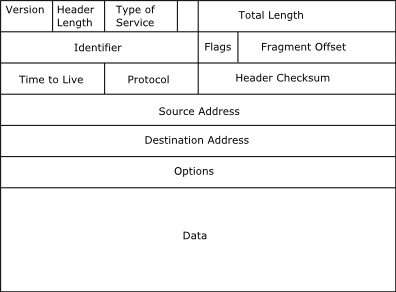
\includegraphics[scale=0.5]{IPv4dg.png}
  \end{center}
\end{figure}

The IP datagram header is 20 bytes, if it carries a TCP datagram, the
size is 40 bytes (in headers).

An IPv4 address consists of 32-bits, and is separted by dots with 8
bits in each space. It is viewed with its decimal representation of
the bits.

The subnet addresses of a network are usually defined with the CIDR
(pronouced cider) notation. The address is written as normal with
x.x.x.x, but with a slash in the end and the number of bits that
define the subnet address. So x.x.x.x/24, as an example.

\subsection{IPv6}
IPv6 is supposed to be the successor of IPv4. The format of an IPv6
datagram can be seen below:

\begin{figure}
  \begin{center}
    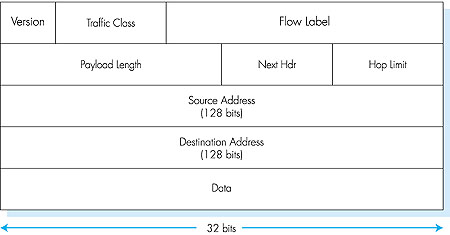
\includegraphics[scale=0.5]{04-40.jpg}
  \end{center}
\end{figure}

The biggest difference is that IPv6 does not allow
fragmentation. Furthermore there is no header checksum, since the
protocols in the transport layer and link layer already check the
sums.

\subsection{IPv4 vs IPv6}
IPv6 is made to be faster than IPv4 by discarding some of the fields
from the IPv4 datagram format, e.g. fragmentation was a time consuming
task. Besides this, the most obvious reason for a change is the limit
of addresses in IPv4 ($2^{32}$), which is almost exhausted. With IPv6,
the address field is 128-bit, making the maximum number of addresses
$2^{128}$. According the estimation based on this calculation,
humanity would not have to increase the number of addresses for a long time.

\subsection{Fragmentation}
Not all link-layer protocols can carry the same amount of data. To
make up for this, an IP datagram can be broken into smaller chunks so
the packet can be delivered. The maximum size of a packet that can be
transmitted is called \textbf{maximum transmission unit} or MTU.

IP keeps track of the packets with the \textit{identification},
\textit{flag}, and \textit{fragmentation offset} fields seen in the
format the datagram.

Note that IPv6 does not allow fragmentation. Instead it encourages
packets to be split, before being sent.
\section{NAT}
NAT (Network Address Translation) is used by routers to control the flow of
packets between the WAN (Wide Area Network) and the LAN. When a user is sitting
behind a router, the router appears to be a communicating client, when the real
client is sitting behind the router. The router maps WAN addresses to LAN
addresses. When a user behind a router wants to communicate with the outside
world, he opens a specific port to communicate over. The outside world only
knows about this port, and sends data to the router through this port. The
router holds a "NAT translation table", which maps open communication from the
WAN to the LAN, so it knows where the incoming data is supposed to go.

\subsection{UPnP}
If an application wants to work around NAT, and the applications end-point of
communication is NAT UPnP compatible (the clients network needs to be
compatible too), the application may create a public IP and a public port, which
appears to be the clients actual IP and port. Other contacts through the
application establish connection through this public mapping, and the router
makes sure it is sent to the correct client.
\section{DHCP}
DHCP is used when a computer wants to connect to a network. It is used
to assign IP addresses to connecting computers.

The computer that wants to connect, sends a DHCP packet to address
0.0.0.0 and the broadcast address 255.255.255.255. The DHCP service
should then give a lease on an address to the connecting
machine. The machine sends a DHCP discover packet, the server answers
with a DHCP offer packet, the machine sends a DHCP request packet, and
finally the server sends a DHCP ACK.

\subsection{CIDR}
CIDR is used to calculate the IP address. The format is x.x.x.x/n
where n ranges from 1 to 32.

To convert from full decimal notation to CIDR notation, we convert the
decimal notation to binary, and note how many bits are set. This
defines what $n$ in the previous example should be.\\
For instance with a subnet mask of 255.255.255.0 would be
255.255.255.0/24 in CIDR notation, since 24 bits are set in the
decimal format.

The other way around, we would have 

\subsection{Forwarding}
\section{Routing}

\section{Distributed Systems}

\section{Security}

\section{Link Layer}

\end{document}
